\documentclass{report}
\usepackage{setspace} % Setting line spacing
\usepackage{ulem} % Underline
\usepackage{caption} % Captioning figures
\usepackage{subcaption} % Subfigures
\usepackage{geometry} % Page layout
\usepackage{multicol} % Columned pages
\usepackage{array,etoolbox}
\usepackage{fancyhdr}
\usepackage{enumitem}
\usepackage[toc,page]{appendix}

% Page layout (margins, size, line spacing)
\geometry{letterpaper, left=1in, right=1in, bottom=1in, top=1in}
\setstretch{1.15}

% Headers
\pagestyle{fancy}
\lhead{PeaPod - Solution Overview}
\rhead{UTAG}

% Metric counter, referencing commands
\newcounter{metricnumber}
\setcounter{metricnumber}{1}
\newcommand{\metricrow}{M\arabic{metricnumber}}
\newcommand{\mlabel}[1]{\addtocounter{metricnumber}{-1}\refstepcounter{metricnumber}\label{#1}\addtocounter{metricnumber}{1}}
\newcommand{\mref}[1]{M\ref{#1}}

\begin{document}

\begin{titlepage}
    \begin{center}
        \vspace*{1.2cm}

        \textbf{\large{PeaPod - Solution Overview}}

        \vspace{0.5cm}

        Outlining a Proposal to the PeaPod Requirements

        \vfill

        Jayden Lefebvre - Lead Engineer\\\small{jayden.lefebvre@mail.utoronto.ca}\\
        \vspace{1cm}
        Nathan Chareunsouk, Navin Vanderwert, Jonas Marshall - Design Engineers

        \vspace{2.5cm}

        Revision 0.3\\
        University of Toronto Agritech\\
        July 3rd, 2021

    \end{center}
\end{titlepage}

\thispagestyle{plain}

\tableofcontents
\newpage

\section{Introduction}
\label{sec:intro}

\subsection{Purpose}
\label{sec:purpose}

The purpose of this document is to outline the fuction and features of a design proposed to meet the PeaPod Requirements.

It accomplishes this by addressing the following prompts on a recursive tree basis:
\begin{enumerate}
    \item \textbf{What} is the design's \uline{purpose} and \uline{function}?
    \item \textbf{How} does it accomplish this? What is the \uline{method/process}?
    \item \uline{Justification} on how the selected features meet the method better than alternatives.
\end{enumerate}

\newpage

\section{Design}

The purpose of the design is derived from the opportunity statement:

PeaPod is "an \uline{automated} and \uline{isolated} \uline{aeroponic} crop growth system, able to generate any \uline{growth environment} from a combination of independent \uline{environment parameters}, with both environment and crop growth \uline{data collection} for \uline{optimization}".

The primary function of the overall design are derived from both the overall purpose as well as the system inputs and outputs as defined by the DSFC Applicant Guide \cite{applicantguide}.

\begin{figure}[h]
    \centering
    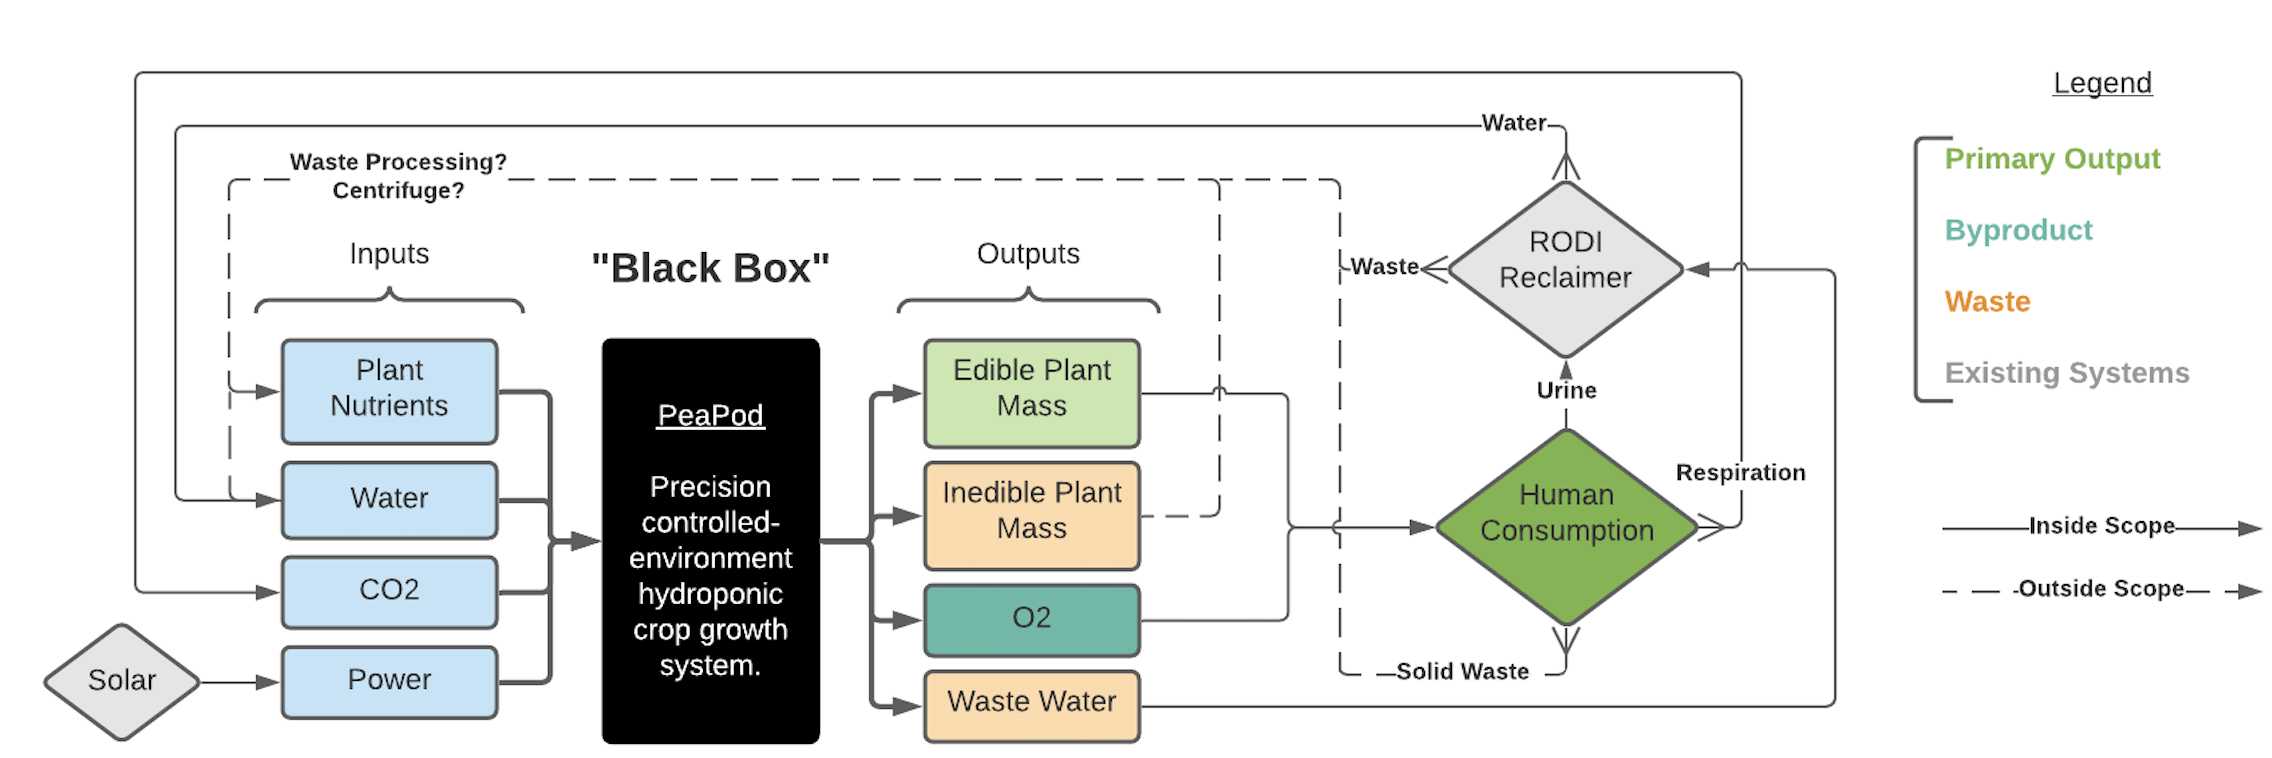
\includegraphics[width=15cm]{images/blackbox.png}
    \hfill
    \caption{"Black box" function diagram of PeaPod.}
\end{figure}

\begin{figure}[h]
    \centering
    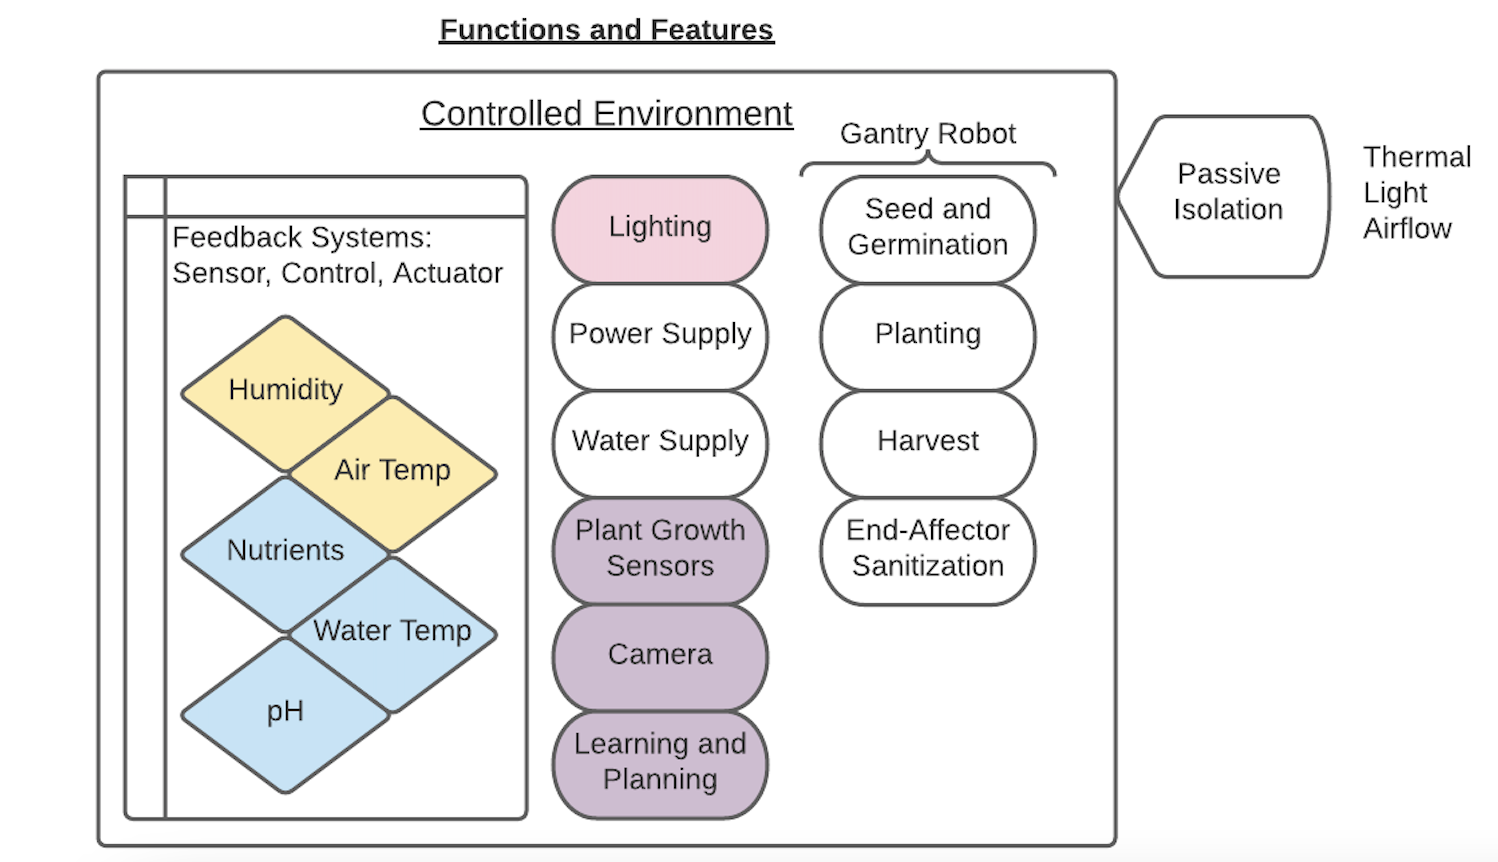
\includegraphics[width=12cm]{images/features.png}
    \hfill
    \caption{Features and feature types of PeaPod.}
\end{figure}

\newpage

\subsection{Automation}
\label{sec:automation}


\textbf{Function}: Performing growth-, maintenance-, and data-related tasks autonomously on the basis of both schedule and necessity to reduce crew maintenance time. Maintains the homogeneity of the internal environment.

\textbf{Process}:
\begin{enumerate}
    \item User inputs program:
    \begin{itemize}
        \item Action-at-timestamp, e.g. lights on at 08:00;
        \item Control target with start/end, e.g. hold air temperature at 22°C from 11:00 to 18:00;
    \end{itemize}
    \item Notification on maintenance requirement (i.e. non-automated input/output management);
    \item "Sense, Plan, Act" robotics/control model:
    \begin{enumerate}
        \item \textit{Senses} current conditions;
        \item \textit{Plans} a path to desired condition;
        \item \textit{Acts} to change current condition to desired condition;
    \end{enumerate}
\end{enumerate}

\textbf{Features}:
\begin{itemize}
    \item Central computer system with internal clock and cloud connection;
    \item Environment sensors (\textit{Sense});
    \item "Program" of time-series and/or control target instructions (\textit{Plan});
    \item Actuators (\textit{Act});
\end{itemize}

\textbf{Justification}: 
\begin{itemize}
    \item \textbf{Function}: Increased accuracy/precision over human interference, minimize human hours spent. Enables control over all parameters simultaneously.
    \item \textbf{Process}: Data structure matches $\vec E$ from the optimization routine (see Section \ref{sec:optimization}). Control loop-style topology is common is well suited for controlled-environment agriculture.
    \item \textbf{Features}: Automation implies computers. Sensors and actuators directly parallel process components.
\end{itemize}

\newpage

\subsection{Housing}
\label{sec:housing}

\textbf{Function}: \textit{Isolates} and \textit{Insulates} growth environment from exterior environment (heat, light, humidity). Provides structural integrity and mounting points for other subsystems (\textit{Frame}).

\textbf{Process}:
\begin{itemize}
    \item Insulation (\textit{keep in}):
    \begin{itemize}
        \item Heat - Insulative/reflective internal shell
        \item Light - Reflective internal shell
        \item Moisture - "Sealed" shell
    \end{itemize}
    \item Isolation (\textit{keep out}):
    \begin{itemize}
        \item Heat - Insulative shell
        \item Light - Opaque shell
        \item Moisture - "Sealed" shell
    \end{itemize}
    \item $\therefore$ Frame skeleton w/ solid, internally-reflective, "sealed" panels;
    \item Standard subframes for mounting entire subsystems modularly;
\end{itemize}

\textbf{Features}:
\begin{itemize}
    \item Aluminum extrusion skeleton w/ standard mounting channels;
    \item Foam insulation panels w/ mylar internal coating slide into exoskeleton channels;
    \item Trays - base subframe unit, adaptable; mounted to vertical internal channels for vertical repositioning:
    \begin{itemize}
        \item Grow trays - Hold up plants, aeroponic nozzles (See \ref{sec:aeroponics}, and misting container.
        \item Lighting trays - Many LED boards, one driver board (See \ref{sec:lighting}).
    \end{itemize}
\end{itemize}

\textbf{Justification}: 
\begin{itemize}
    \item \textbf{Function}: Insulation increases thermal and light efficiency. Isolation increases safety against cross-contamination, pathogens, harmful substances.
    \item \textbf{Process}: Solid frame-and-panel construction is efficient for packing away, and is honestly just simple. Adaptable tray subframes make future feature development easier, and allows to modularly swap subsystems.
    \item \textbf{Features}: Aluminum extrusion is commonly used for frames. Allows strong, repositionable mounting via channels. Foam insulation is highly insulative and opaque, and mylar ensures internal light reflection. Sliding directly into extrusion channels boosts "seal".
\end{itemize}

\newpage

\subsection{Aeroponics}
\label{sec:aeroponics}

\textbf{What}: Medium-free growing method that uses nutrients dissolved within atomized water.

\textbf{How}: High-pressure nozzles deliver atomized nutrient solution to plant roots. Uses parallel distribution topology.
\begin{itemize}
    \item Pump fills tank with water that has nutrients dissolved within;
    \item Tank uses an air bladder to hold water at desired PSI;
    \item Switch checks line pressure and activates/deactivates pump to maintain PSI;
    \item Solenoid ball valve feeds water to nozzle;
    \item Nozzle atomizes water to $\approx$50 micron droplets;
    \item T-quick connects with solenoid ball valves at every unit height feed individual trays;
\end{itemize}

\textbf{Why}: No water parameter feedback, 98\% more water efficient, minimizes pathogens and waste water.

\subsection{Environment Control}
\label{sec:environment}

The environment control feature can be broken up into \textbf{control systems} (\ref{sec:airtemp}-\ref{sec:dehum}; sometimes in two parts) and \textbf{set systems} (\ref{sec:watertemp}-\ref{sec:lighting}).

\subsubsection{Air Temperature}
\label{sec:airtemp}

\textbf{What}: Maintaining desired air temperature within the enclosure.

\textbf{How}: Thermoelectric heating/cooling system (peltier tiles w/ polarity switch, 'dimming' current control, PID) on a heat sink w/ fan, feedback from distributed temp sensors.

\textbf{Why}: TECs have better space and energy efficiency, less complexity (no liquids, pressurized fluids, etc.), better control vs other methods. PID provides best control.

\newpage

\subsubsection{Air Humidification}
\label{sec:airhum}

\textbf{What}: Adding water vapour to air.

\textbf{How}: Ultrasonic nebulizer (piezo disc w/ custom driver circuit), RO water.

\textbf{Why}: Piezo for droplet size, commonly used; RO for purity of water vapour.

\subsubsection{Air Dehumidification}
\label{sec:dehum}

\textbf{What}: Absorbs water vapour from the air.

\textbf{How}: Silica gel bead cartridges with fans/valves to control airflow across.

\textbf{Why}: Non-toxic, safe, cheap, effective. Color-changing indication at saturation, easily reset by baking and recapturing water.

\subsubsection{Solution Temperature}
\label{sec:watertemp}

\textbf{What}: Maintaining desired water temperature within the water store.

\textbf{How}: Same as \ref{sec:airtemp}; on a water block.

\textbf{Why}: Same as \ref{sec:airtemp}.

\subsubsection{Solution Nutrients}
\label{sec:nutrients}

\textbf{What}: Precisely dosing the correct amount of various nutrients (K${}^+$, NO${}_3^-$, etc.) to the water system at setup/water addition.

% TODO: List of nutrients?

\textbf{How}: Syringe-like dosage via servo motor to set ppm based on fill volume.

\textbf{Why}: Syringe dosage is precise, easy to refill.

\subsubsection{Solution pH}
\label{sec:ph}

\textbf{What}: Precisely adds pH up/down solutions to set the solution pH at setup/water addition.

\textbf{How}: Same as \ref{sec:nutrients}.

\textbf{Why}: Same as \ref{sec:nutrients}.

\newpage

\subsubsection{Lighting}
\label{sec:lighting}

\textbf{What}: Wide spectrum precision LED lighting targeting PAR.

\textbf{How}: N LED series/colors, N controlled-current PWM drivers, M LEDs per series = NxM LEDs. Custom LED boards wired in series, one power board per tray, w/ diffusion.

\textbf{Why}: LED > every other type in every way, PWM easy protocol, CC because they’re LEDs.

% \textbf{What}: 
% \textbf{How}: 
% \textbf{Why}:

\subsection{Optimization}
\label{sec:optimization}

\textbf{Function}: Continuously improve yield/etc. of crops as more environment parameter and crop metric data is gathered.

\textbf{Process}: 

Assume a plant's growth rate (or state change) is related to its current internal state $\vec P \in \R^n$ (for $n$ plant metrics) and the environment conditions $\vec E \in \R^m$ (for $m$ environment parameters). Let these both be functions $\vec P (t),\vec E(t)$ defined at each $t$, where $t=0$ indicates the time of planting. Assume that this relationship is constant for all members of a given species.

Define plant state change $\vec P'$: 

$$\vec P'(t) = \frac{d}{dt}\vec P(t)$$

Define the plant-environment behaviour function $Q$: 

$$Q(\vec P(t), \vec E(t), t)=\vec P'(t)$$ 

Aka given the current internal and external states, determine the plant's state change.

By setting $\vec E_{set}(t)~\forall~ t$, recording $\vec P(t)~\forall~ t$ and $\vec E(t)\approx \vec E_{set}(t)~\forall~ t$ (See \ref{sec:environment}), and calculating $\vec P'(t)~\forall~ t$, we can fit $\vec Q$ to our data.

By fitting $\vec Q$, we can predict $\vec P$ at any $\vec E$ and $t$. For example:

$$\vec P(t+\Delta t)=P(t)+\Delta t\cdot Q(\vec P(t),\vec E(t))$$

\textbf{Features}:
\begin{itemize}
    \item Machine learning model to represent $Q$
    \item Environment sensors to collect $\vec E$
    \item Plant metrics to collect $\vec P$
\end{itemize}

\newpage

% References
\bibliographystyle{IEEEtran}
\bibliography{references}
\end{document}